\section{Discussion}

\subsection{Does the model learn grounded representations?}

A natural question to ask if whether the multitask model is actually learning representations that are relevant for the images. We answer this question by evaluating the Imaginet decoder in an image--sentence ranking task. Here the input is a source language sentence, from which we predict its image vector $\mathbf{\hat{v}}$. The predicted vector $\mathbf{\hat{v}}$ can be compared against the true image vectors $\mathbf{v}$ in the evaluation data using the cosine distance to produce a ranked order of the images. Our model returns a median rank of 11.0 for the true image compared to the predicted image vector.
Figure \ref{fig:discussion:examples} shows examples of the nearest neighbours of the images predicted by our multitask model. We can see that the combination of the multitask source language representations and {\sc imaginet} decoder
leads to the prediction of relevant images. This confirms that the shared encoder is indeed learning visually grounded representations.

\subsection{The effect of visual feature vectors}

\begin{figure*}
 \begin{subfigure}[b]{1\textwidth}
 \centering
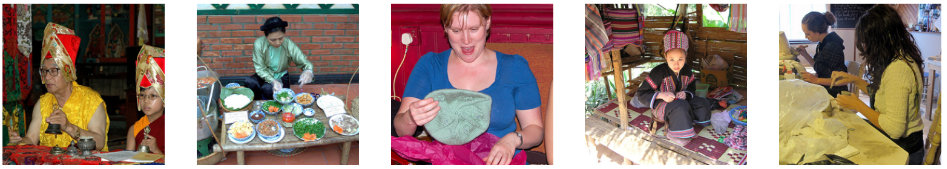
\includegraphics[width=0.75\textwidth]{chapters/IJCNLP/images/dev_example_notext.png}
\caption{Nearest neighbours for ``a native woman is working on a craft project .''}
\vspace{2ex}
\end{subfigure}
 \begin{subfigure}[b]{1\textwidth}
 \centering
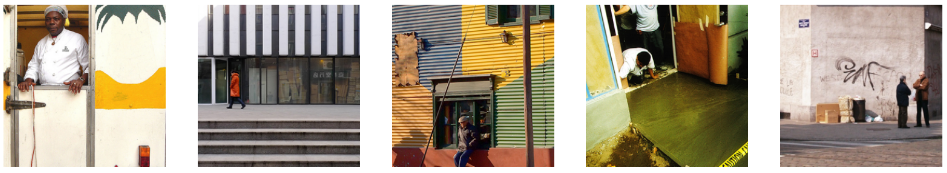
\includegraphics[width=0.75\textwidth]{chapters/IJCNLP/images/dev_example2_notext.png}
\caption{Nearest neighbours for ``there is a cafe on the street corner with an oval painting on the side of the building .''}
\end{subfigure}
\caption{We can interpret the {\sc imaginet} Decoder by visualising the predictions made by our model.}\label{fig:discussion:examples}
\end{figure*}

We now study the effect of varying the Convolutional Neural Network used to extract the visual features used in the Imaginet decoder.
It has previously been shown that the choice of visual features can affect the performance of vision and language models \citep{Jabri2016,Kiela2016}.
We compare the effect of training the {\sc imaginet} decoder to predict different types of image features, namely: 4096D features extracted from the `fc7`' layer of the VGG-19 model \citep{simonyan2014very}, 2048D features extracted from the `pool5/7x7\_s1' layer of InceptionNet V3 \citep{Szegedy2015}, and 2048D features extracted from `avg\_pool` layer of ResNet-50 \citep{he2016deep}.
Table \ref{tab:results:features} shows the results of this experiment.
There is a clear difference between predicting the 2048D vectors (Inception-V3 and ResNet-50) compared to the 4096D vector from VGG-19).
This difference is reflected in both the translation Meteor score and the Median rank of the images in the validation dataset. This is likely because it is easier to learn the parameters of the image prediction model that has fewer parameters (8.192 million for VGG-19 vs. 4.096 million for Inception-V3 and ResNet-50).
However, it is not clear why there is such a pronounced difference between the Inception-V3 and ResNet-50 models\footnote{We used pre-trained CNNs (\url{https://github.com/fchollet/deep-learning-models}), which claim equal ILSVRC object recognition performance for both models: 7.8\% top-5 error with a single-model and single-crop.}.

\begin{table}
\centering
\renewcommand{\arraystretch}{1.3}
\begin{tabular}{lcc}
\toprule
& Meteor & Median Rank \\
\midrule
Inception-V3 & 56.0 $\pm$ 0.1 & 11.0 $\pm$ 0.0\\
Resnet-50 & 54.7 $\pm$ 0.4 & 11.7 $\pm$ 0.5 \\
VGG-19 & 53.6 $\pm$ 1.8 & 13.0 $\pm$ 0.0 \\
\bottomrule
\end{tabular}
\caption{The type of visual features predicted by the {\sc imaginet} Decoder has a strong impact on the Multitask model performance.}\label{tab:results:features}
\end{table}
